\subsection{Kapselung Versatile IKE Configuration Interface}
Wie erwähnt bietet die strongSwan Open Source VPN Software das Versatile
IKE Configuration Interface (VICI) \cite{vici} an, welche es erlaubt eine Management Anwendung über ein C, Ruby, Python oder Perl Binding an den Charon
IKE Daemon anzubinden.\\
Um die VICI-Schnittstelle zu verwenden, kann es es einfach via PIP installiert werden.\\
\begin{lstlisting}[style=BashInputStyle]
	pip install vici==5.4.1dev3
\end{lstlisting}
\medskip

\subsubsection{Kommunikation}
\noindent
\begin{minipage}[t]{0.5\textwidth}
    \vspace{0pt}
    \begin{figure}[H]
        \centering
        \includegraphics[width=200pt]{images/vici_wrapper_overview.png}
        \caption[VICI Übersicht]{Vici Übersicht}
    \end{figure}
    \hfill
\end{minipage}   
\noindent\begin{minipage}[t]{0.5\textwidth}
\vspace{0pt}
Die Kommunikation, welche durch die Schnittstelle angeboten wird, basiert auf einem Unix Socket (AF\_UNIX). Dabei wird in Python die OrderedDictionary-Klasse verwendet, die als verschachtelte Property List für die Konfigurationsparameter dient. \\
\end{minipage}
\hfill


\paragraph{ordered Dictionaries}\label{orderedDictionary}sind folgendermassen strukturiert:
\begin{python}
OrderedDict([
	('cert', OrderedDict([
		('remote_addrs', ['gateway'])
	)])
])
\end{python}

\subsubsection{ViciWrapper}
\noindent
\begin{minipage}[t]{0.5\textwidth}
    \vspace{0pt}
Um das VICI Plugin von unserem Code zu trennen, haben wir eine Wrapperklasse darum herum geschrieben. Dies verringert die Kopplung, ermöglicht uns eigene Exception zu werfen und gewisse Aufrufe zu kombinieren. \\
Die Hauptfunktionen des Wrappers sind:
\begin{itemize}
    \item Auf- und Abbau der Sockets
    \item Übertragen der Verbindungskonfigurationen
    \item Initialisieren und Terminieren der Tunnels
    \item Auslesen von Statusinformationen
    \item Auslesen der strongSwan Konfiguration
\end{itemize}
    \hfill
\end{minipage}   
\noindent\begin{minipage}[t]{0.5\textwidth}
\vspace{0pt}
        \begin{figure}[H]
        \centering
        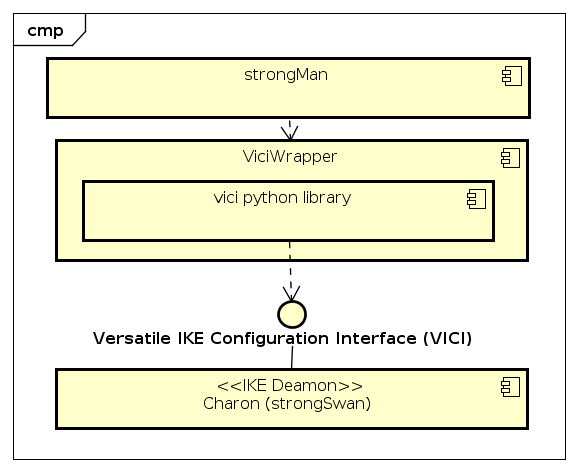
\includegraphics[width=200pt]{images/vici_wrapper.png}
        \caption[VICI Diagramm]{VICI Diagramm}
        \end{figure}
        \medskip
\end{minipage}
\hfill














